% !TEX root = /media/ueslei/Ueslei/INPE/PCI/Guia_COAWST/main.tex
\chapterimage{ocean2.jpg}
\chapter{Construindo o ROMS}\index{Contruindo o ROMS}
\section{Instalando as bibliotecas do Python no computador pessoal}
\bigskip

\noindent Antes de gerar os arquivos de condições e a grade para o ROMS, é necessário instalar as bibliotecas e dependências. Nesta seção serão disponibilizados os endereços para baixá-las, bem como os comandos no terminal via \textit{apt-get}.
\bigskip

\noindent Existem duas maneiras de instalar as bibliotecas necessárias: de modo manual, e através do Anaconda. Este último é uma plataforma gratuita e de código aberto para Python e R e possui um gerenciador de pacotes chamado Conda, que facilita a instalação de bibliotecas. Neste guia, apresentarei as duas opções. Pela praticidade, sugiro instalar usando o Conda (Seção \textcolor{bleu_cite}{\ref{condasec}}), porém cuidado para conflito de versões, poise os repositórios do Conda são atualizados constantemente.
\bigskip

\begin{tcolorbox}[enhanced,
  grow to left by   = 0cm,
  grow to right by  = 0cm,
  enlarge top by    = 0cm,
  enlarge bottom by = 0cm,
  tcbox raise base,
  boxrule           = 1.0pt,
  left              = 18mm,
  colframe          = red!50!black,coltext=red!25!black,colback=red!10!white,
  overlay           = {\begin{tcbclipinterior}\fill[red!75!blue!50!white] (frame.south west)
    rectangle node[text=white,font=\sffamily\bfseries\footnotesize,rotate=0] {ATENÇÃO} ([xshift=18mm]frame.north west);\end{tcbclipinterior}}]
A construção do ROMS deverá ser feita no seu próprio computador e não mais no Kerana, como feito anteriormente com o WRF.
\end{tcolorbox}
\bigskip

\subsection{Instalação manual}\index{Instalação manual}
\bigskip
\noindent Abra o terminal, e crie uma pasta na sua \textit{home} chamada \textit{libsmodels}. Nela serão adiconados os arquivos baixados e as bibliotecas.
\bigskip

\begin{bashcode}
sudo mkdir libsmodels
\end{bashcode}
\bigskip

\noindent Caso não tenha o \textit{gfortran} e o \textit{g++} instalados, instale via \textit{apt-get}.
\bigskip
\begin{bashcode}
sudo apt-get install gfortran
sudo apt-get install g++
\end{bashcode}
\bigskip

\noindent A seguir, baixe o OpenMPI 2.0.1 (\textcolor{bleu_cite}{\textit{https://www.open-mpi.org/software/ompi/v2.0/}}), extraia o arquivo dentro da pasta \textit{libsmodels} e digite no terminal:
\bigskip

\begin{bashcode}
export F77=gfortran
export FC=gfortran
export FC=gfortran
export CC=gcc
export CXX=g++
export FFLAGS="-m64 -fdefault-integer-8"
export FCFLAGS="-m64 -fdefault-integer-8"
export CFLAGS=-m64
export CXXFLAGS=-m64
\end{bashcode}
\bigskip

\noindent Entre na pasta do OpenMPI e digite:
\bigskip

\begin{tcolorbox}[enhanced,
  grow to left by   = 0cm,
  grow to right by  = 0cm,
  enlarge top by    = 0cm,
  enlarge bottom by = 0cm,
  tcbox raise base,
  boxrule           = 1.0pt,
  left              = 18mm,
  colframe          = red!50!black,coltext=red!25!black,colback=red!10!white,
  overlay           = {\begin{tcbclipinterior}\fill[red!75!blue!50!white] (frame.south west)
    rectangle node[text=white,font=\sffamily\bfseries\footnotesize,rotate=0] {ATENÇÃO} ([xshift=18mm]frame.north west);\end{tcbclipinterior}}]
Altere o nome do computador abaixo (\textit{usuario}) pelo nome do seu computador.
\end{tcolorbox}
\bigskip

\begin{bashcode}
./configure --prefix=/home/usuario/libsmodels
sudo make
sudo make check
sudo make install
\end{bashcode}
\bigskip

\noindent Volte até a sua \textit{/home/usuario} e abra o arquivo oculto \textit{.bashrc} através do comando \textit{gedit .bashrc} ou com o editor de texto de sua preferência e nas linhas finais do arquivo escreva:
\bigskip

\begin{bashcode}
export PATH=/home/usuario/libsmodels/bin:$PATH
export LD_LIBRARY_PATH=/home/usuario/libsmodels/lib:$LD_LIBRARY_PATH
export PATH=/home/usuario/libsmodels/include:$PATH
\end{bashcode}
\bigskip

\noindent Salve o arquivo e no terminal, digite o comando a seguir para atualizar o arquivo e aplicar as mudanças.
\bigskip

\begin{bashcode}
source .bashrc
\end{bashcode}
\bigskip

\noindent Para testar se a instalação do OpenMPI está correta, digite no terminal:
\bigskip

\begin{bashcode}
ompi_info -a grep 'Fort integer size'
\end{bashcode}
\bigskip

\noindent O resultado deverá ser:
\bigskip

\begin{bashcode}
Fort integer size: 8
\end{bashcode}
\bigskip

\noindent Caso não tenha instalado no seu computador, será necessário instalar o \textit{m4}, \textit{make} e \textit{perl}. Para checar se o seu computador já possui estes programas instalados:
\bigskip

\begin{bashcode}
which m4
which make
which perl
\end{bashcode}
\bigskip

\noindent Caso a resposta seja negativa, instale a partir dos comandos a seguir:
\bigskip

\begin{bashcode}
sudo apt-get install m4
sudo apt-get install make
sudo apt-get install perl
\end{bashcode}
\bigskip

\noindent Instale o \textit{szip 2.1} (\textcolor{bleu_cite}{\textit{https://www.hdfgroup.org/HDF5/release/obtain5.html}}). Baixe-o, descompacte na pasta \textit{/home/usuario/libsmodels} e entre, via terminal, na pasta do \textit{szip} digite:
\bigskip

\begin{bashcode}
export F77=gfortran
export FC=gfortran
export CC=gcc
export CXX=g++
export FFLAGS="-m64 -fdefault-integer-8"
export FCFLAGS="-m64 -fdefault-integer-8"
export CFLAGS=-m64
export CXXFLAGS=-m64
./configure --prefix=/home/usuario/libsmodels
sudo make
sudo make check
sudo make install
\end{bashcode}
\bigskip

\noindent Instale o \textit{zlib 1.2.8} (\textcolor{bleu_cite}{\textit{http://zlib.net/}}). Baixe-o, descompacte na pasta \textit{/home/usuario/libsmodels} e entre, via terminal, na pasta do \textit{zlib} digite:
\bigskip

\begin{bashcode}
export F77=gfortran
export FC=gfortran
export CC=gcc
export CXX=g++
export FFLAGS="-m64 -fdefault-integer-8"
export FCFLAGS="-m64 -fdefault-integer-8"
export CFLAGS=-m64
export CXXFLAGS=-m64
./configure --prefix=/home/usuario/libsmodels
sudo make
sudo make check
sudo make install
\end{bashcode}
\bigskip

\noindent Instale agora o \textit{Curl 7.50.3} (\textcolor{bleu_cite}{\textit{http://curl.haxx.se/download.html}}). Baixe-o, descompacte na pasta \textit{/home/usuario/libsmodels} e entre, via terminal, na pasta do \textit{Curl} digite:
\bigskip

\begin{bashcode}
export F77=gfortran
export FC=gfortran
export CC=gcc
export CXX=g++
export FFLAGS="-m64 -fdefault-integer-8"
export FCFLAGS="-m64 -fdefault-integer-8"
export CFLAGS=-m64
export CXXFLAGS=-m64
./configure --prefix=/home/usuario/libsmodels/
sudo make
sudo make check
sudo make install
\end{bashcode}
\bigskip

\noindent Instale as bibliotecas necessárias para usar o HDF5. Digite:
\bigskip

\begin{bashcode}
sudo apt-get install libgtk2.0-dev
\end{bashcode}
\bigskip

\noindent Instale o \textit{HDF5 1.8.9} (\textcolor{bleu_cite}{\textit{https://www.hdfgroup.org/HDF5/release/obtain5.html}}). Baixe-o, descompacte na pasta \textit{/home/usuario/libsmodels} e entre, via terminal, na pasta do \textit{HDF5} digite:
\bigskip

\begin{bashcode}
export FC=gfortran
export CC=gcc
export CXX=g++
export LDFLAGS=-L/home/usuario/libsmodels/lib
export CPPFLAGS=-I/home/usuario/libsmodels/include
\end{bashcode}
\bigskip

\noindent Na mesma linha de comando, digite:
\bigskip

\begin{bashcode}[fontsize=\footnotesize]
./configure --enable-fortran=yes --enable-fortran2003=yes --enable-cxx=yes
--with-szlib=/home/usuario/libsmodels --with-zlib=/home/usuario/libsmodels --enable-hl
--enable-shared --prefix=/home/usuario/libsmodels
\end{bashcode}
\bigskip

\noindent Complete a instalação do \textit{HDF5} com os comandos abaixo:
\bigskip

\begin{bashcode}
sudo make
sudo make check
sudo make install
\end{bashcode}
\bigskip

\noindent O próximo passo é instalar o \textit{NetCDF-C 4.4.1} (\textcolor{bleu_cite}{\textit{https://www.unidata.ucar.edu/downloads/netcdf/index.jsp}}). Baixe-o, descompacte na pasta \textit{/home/usuario/libsmodels} e na pasta do \textit{NetCDF-C} digite:
\bigskip

\begin{bashcode}[fontsize=\scriptsize]
export FC=gfortran
export CC=gcc
export CXX=g++
export LDFLAGS=-L/home/usuario/libsmodels/lib
export CPPFLAGS=-I/home/usuario/libsmodels/include
\end{bashcode}
\bigskip

\noindent Na mesma linha de comando, digite:
\bigskip

\begin{bashcode}[fontsize=\scriptsize]
./configure --prefix=/home/usuario/libsmodels
--enable-netcdf4 --with-hdf5=/home/usuario/libsmodels --enable-shared --enable-dap
\end{bashcode}
\bigskip

\noindent Complete a instalação do \textit{NetCDF-C} com os comandos abaixo:
\bigskip

\begin{bashcode}
sudo make
sudo make check
sudo make install
\end{bashcode}
\bigskip

\noindent Instale agora o \textit{NetCDF-Fortran 4.2} (\textcolor{bleu_cite}{\textit{https://www.unidata.ucar.edu/downloads/netcdf/index.jsp}}). Baixe-o, descompacte na pasta \textit{/home/usuario/libsmodels} e na pasta do \textit{NetCDF-Fortran} digite:
\bigskip

\begin{bashcode}[fontsize=\scriptsize]
export FC=gfortran
export F77=gfortran
export CC=gcc
export CXX=g++
export LDFLAGS=-L/home/usuario/libsmodels/lib
export CPPFLAGS=-I/home/usuario/libsmodels/include
export LIBS='-lnetcdf -lhdf5 -lhdf5_hl -lz'
\end{bashcode}
\bigskip

\noindent Na mesma linha de comando, digite:
\bigskip

\begin{bashcode}
./configure --prefix=/home/usuario/libsmodels --enable-netcdf4
--with-hdf5=/home/usuario/libsmodels --enable-shared --enable-dap
\end{bashcode}
\bigskip

\noindent Termine a instalação do \textit{NetCDF-Fortran}:
\bigskip

\begin{bashcode}
sudo make
sudo make check
sudo make install
\end{bashcode}
\bigskip

\noindent Instale o \textit{JasPer 1.900.1} (\textcolor{bleu_cite}{\textit{http://www.linuxfromscratch.org/blfs/view/svn/general/jasper.html}}). Baixe-o, descompacte na pasta \textit{/home/usuario/libsmodels} e na pasta do JasPer digite:
\bigskip

\begin{bashcode}
export FC=gfortran
export F77=gfortran
export CC=gcc
export CXX=g++
./configure --prefix=/home/usuario/libsmodels
sudo make
sudo make check
sudo make install
\end{bashcode}
\bigskip

\noindent Instale o \textit{libpng 1.6.24} (\textcolor{bleu_cite}{\textit{http://sourceforge.net/projects/libpng/?source=typ\_redirect}}). Baixe-o, descompacte na pasta \textit{/home/usuario/libsmodels} e na pasta do \textit{libpng} digite:
\bigskip

\begin{bashcode}[fontsize=\scriptsize]
export FC=gfortran
export F77=gfortran
export CC=gcc
export CXX=g++
export LDFLAGS=-L/home/usuario/libsmodels/lib
export CPPFLAGS=-I/home/usuario/libsmodels/include
export LIBS='-lz'
./configure --with-zlib=/home/usuario/libsmodels --prefix=/home/usuario/libsmodels
sudo make
sudo make check
sudo make install
\end{bashcode}
\bigskip

\noindent Instale o \textit{Udunits 2.1.24} (\textcolor{bleu_cite}{\textit{ftp://ftp.unidata.ucar.edu/pub/udunits/}}).  Baixe-o, descompacte na pasta \textit{/home/usuario/libsmodels} e entre na pasta do \textit{Udunits} digite:
\bigskip

\begin{bashcode}
export FC=gfortran
export F77=gfortran
export CC=gcc
export CXX=g++
./configure --prefix=/home/usuario/libsmodels
sudo make
sudo make check
sudo make install
\end{bashcode}
\bigskip

\noindent Instale o NetCDF4 para Python. Neste caso, baixe primeiramente o Git e use-o para baixar.
\bigskip

\begin{bashcode}
sudo apt-get install git
\end{bashcode}
\bigskip

\noindent Clone o repositório do \textit{NetCDF4-Python} com o comando:
\bigskip

\begin{bashcode}
git clone https://github.com/Unidata/netcdf4-python
\end{bashcode}
\bigskip

\noindent Entre na pasta do NetCDF4-Python e modifique o arquivo \textit{setup.cfg.template} e salve:
\bigskip

\begin{bashcode}
ncconfig    = /home/usuario/libsmodels/bin/nc-config
netCDF4_dir = /home/usuario/libsmodels
HDF5_dir    = /home/usuario/libsmodels
szip_dir    = /home/usuario/libsmodels
jpeg_dir    = /home/usuario/libsmodels
curl_dir    = /home/usuario/libsmodels
\end{bashcode}
\bigskip

\noindent Modifique o nome do arquivo \textit{setup.cfg.template} para setup.cfg:
\bigskip

\begin{bashcode}
mv setup.cfg.template setup.cfg
\end{bashcode}
\bigskip

\noindent Crie na pasta \textit{libsmodels} as subpastas \textit{lib/python2.7/site-packages}:
\bigskip

\begin{bashcode}
mkdir lib
cd lib
mkdir python2.7
cd python2.7
mkdir site-packages
\end{bashcode}
\bigskip

\noindent Volte para a pasta principal do \textit{NetCDF4-Python} e compile:
\bigskip

\begin{bashcode}
python setup.py build
python setup.py install --prefix=/home/usario/libsmodels
\end{bashcode}
\bigskip

\noindent Caso queira conferir se a instalação ocorreu com sucesso, tente importar a biblioteca no Python. Digite no terminal:
\bigskip

\begin{bashcode}
python
import netCDF4
\end{bashcode}
\bigskip

\noindent Instale agora o \textit{mpi4py} (\textcolor{bleu_cite}{\textit{https://pypi.python.org/pypi/mpi4py)}}, extraia e digite:
\bigskip

\begin{bashcode}
python setup.py build
python setup.py install --prefix=/home/usuario/libsmodels
\end{bashcode}
\bigskip

\noindent Para testar a instalação, digite:
\bigskip

\begin{bashcode}
mpiexec -n 5 python demo/helloworld.py
\end{bashcode}
\bigskip

\noindent Instale agora o \textit{ESMF} e \textit{ESMPy} (\textcolor{bleu_cite}{\textit{https://www.earthsystemcog.org/projects/esmpy/releases}}). Primeiro digite os comandos a seguir para instalar os arquivos de bibliotecas necessárias:
\bigskip

\begin{bashcode}
sudo apt-get install python-setuptools
sudo easy_install pip
sudo pip install distribute
sudo pip install nose
\end{bashcode}
\bigskip

\noindent Dentro da pasta do ESMF, digite no terminal:
\bigskip

\begin{bashcode}[fontsize=\footnotesize]
export ESMF_F90COMPILER=gfortran
export ESMF_NETCDF_LIBS="-lnetcdff -lnetcdf"
export ESMF_DIR=/home/usuario/libsmodels/packages/esmp.ESMF_6_3_0rp1_ESMP_01/esmf
export ESMF_NETCDF="local"
export ESMF_COMPILER=gfortran
export ESMF_COMM=openmpi
export ESMF_TESTEXHAUSTIVE=on
export ESMF_TESTSHAREDOBJ=on
export ESMF_NETCDF_INCLUDE=/home/usuario/libsmodels/include
export ESMF_NETCDF_LIBPATH=/home/usuario/libsmodels/lib
export ESMF_INSTALL_PREFIX=/home/usuario/libsmodels/ESMF
make
make check
make all_tests
make install
\end{bashcode}
\bigskip

\noindent Entre na pasta \textit{scr/addon/ESMPy}:
\bigskip

\begin{bashcode}[fontsize=\scriptsize]
cd src/addon/ESMPy/
\end{bashcode}
\bigskip

\noindent Na mesma linha de comando, digite:
\bigskip

\begin{bashcode}[fontsize=\footnotesize]
python setup.py build
--ESMFMKFILE=/home/usuario/libsmodels/ESMF/lib/libO/Linux.gfortran.64.openmpi.default/esmf.mk
\end{bashcode}
\bigskip

\noindent Complete a instalação:
\bigskip

\begin{bashcode}
python setup.py install --prefix=/home/usuario/libsmodels
python setup.py test
\end{bashcode}
\bigskip

\noindent Instale o Octant, utilizando o Git:
\bigskip

\begin{bashcode}
git clone https://github.com/hetland/octant
\end{bashcode}
\bigskip

\noindent Na pasta \textit{octant/external}, exclua tudo e baixe os seguintes arquivos:
\bigskip

\begin{bashcode}
rm -rf *
git clone https://github.com/sakov/gridgen-c.git
git clone https://github.com/sakov/gridutils-c
git clone https://github.com/sakov/csa-c
git clone https://github.com/sakov/nn-c
\end{bashcode}
\bigskip

\noindent E renomeie as pastas baixadas para, respectivamente: \textit{gridgen}, \textit{gridutils}, \textit{csa} e \textit{nn}. Entre na pasta \textit{nn/nn}, exporte as bibliotecas e instale o \textit{nn}:
\bigskip

\begin{bashcode}
cd nn/nn/
export FC=gfortran
export F77=gfortran
export CC=gcc
export CXX=g++
./configure --prefix=/home/usuario/libsmodels
make
make install
\end{bashcode}
\bigskip

\noindent Instale o \textit{csa} da mesma maneira que foi instalado o nn:
\bigskip

\begin{bashcode}
cd ../../csa/csa/
export FC=gfortran
export F77=gfortran
export CC=gcc
export CXX=g++
./configure --prefix=/home/usuario/libsmodels
make
make install
\end{bashcode}
\bigskip

\noindent Ainda na pasta do \textit{csa}, compie o arquivo \textit{csa.o} para a pasta \textit{/home/usuario/libsmodels/lib}:
\bigskip

\begin{bashcode}
cp csa.o /home/usuario/libsmodels/lib/l
\end{bashcode}
\bigskip

\noindent Instale o \textit{gridutils}:
\bigskip

\begin{bashcode}[fontsize=\scriptsize]
cd ../../gridutils/gridutils/
export FC=gfortran
export F77=gfortran
export CC=gcc
export CXX=g++
LDFLAGS=-L/home/usuario/libsmodels/lib
./configure --prefix=/home/usuario/libsmodels CPPFLAGS=-I/home/usuario/libsmodels/include
make
make install
\end{bashcode}
\bigskip

\noindent Instale o \textit{gridgen}:
\bigskip
\begin{bashcode}[fontsize=\scriptsize]
cd ../../gridgen/
export FC=gfortran
export F77=gfortran
export CC=gcc
export CXX=g++
LDFLAGS=-L/home/usuario/libsmodels/lib
./configure -prefix=/home/usuario/libsmodels CPPFLAGS=-I/home/usuario/libsmodels/include
\end{bashcode}
\bigskip

\noindent Abra o arquivo \textit{makefile} e altere no arquivo de acordo com o que está abaixo:
\bigskip

\begin{bashcode}
CFLAGS = -g -O2 -Wall -I/home/usuario/libsmodels/include
LDFLAGS = -L/home/usuario/libsmodels/lib
LIBS = -lgu -lm -L/home/usuario/libsmodels/lib
\end{bashcode}
\bigskip

\noindent Salve o arquivo, feche e digite no terminal:
\bigskip

\begin{bashcode}
make
make lib
make shlib
make install
\end{bashcode}
\bigskip

\noindent Dentro da pasta \textit{/home/usuario/libsmodels/octant/octant}, modifique o arquivo \textit{grid.py} como o exemplo abaixo (aproximadamente na linha 898).
\bigskip

\begin{tcolorbox}[enhanced,
  grow to left by=0cm,%   equivalent to negative mdframed 'leftmargin'
  grow to right by=0cm,%  equivalent to negative mdframed 'rightmargin'
  enlarge top by=0cm,%     equivalent to mdframed 'skipabove'
  enlarge bottom by=0cm,%  equivalent to mdframed 'skipbelow'
  tcbox raise base,
  boxrule=1.0pt,
  left=18mm,
  colframe=red!50!black,coltext=red!25!black,colback=red!10!white,
  overlay={\begin{tcbclipinterior}\fill[red!75!blue!50!white] (frame.south west)
    rectangle node[text=white,font=\sffamily\bfseries\footnotesize,rotate=0] {ATENÇÃO} ([xshift=18mm]frame.north west);\end{tcbclipinterior}}]
Observe atentamente para o espaço em branco antes do início do texto, pois poderá dar erro na hora de instalar se a contagem de linha estiver errada.
\end{tcolorbox}
\bigskip


\begin{bashcode}[fontsize=\footnotesize]
self._libgridgen = np.ctypeslib.load_library('libgridgen.so', '/home/usuario/libsmodels/lib')
print octant.__path__[0]
self._libgridgen = np.ctypeslib.load_library('_gridgen', octant.__path__[0])
\end{bashcode}
\bigskip

\noindent Salve e feche o arquivo. Digite agora:
\bigskip

\begin{bashcode}
python setup.py build --fcompiler=gfortran
\end{bashcode}
\bigskip

\noindent Em \textit{/home/usuario/libsmodels/octant/octant}, abra o arquivo \textit{csa.py} e modifique como abaixo, observando corretamente o espaçamento:
\bigskip

\begin{bashcode}
_csa = np.ctypeslib.load_library('csa.o', '/home/usuario/libsmodels/libs')
\end{bashcode}
\bigskip

\noindent Por fim, em \textit{/home/usuario/libsmodels/octant}, digite:
\bigskip

\begin{bashcode}
python setup.py install --prefix=/home/usuario/pythonmodels/octant
\end{bashcode}
\bigskip

\noindent Adicione os diretórios no seu \textit{.bashrc}. Lembrando novamente que o \textit{.bashrc} encontra-se na sua \textit{/home/usuario}.
\bigskip

\begin{bashcode}[fontsize=\scriptsize]
export PYTHONPATH=$PYTHONPATH:/home/usuario/libmodels/octant
export PYTHONPATH=$PYTHONPATH:/home/usuario/libmodels/octant/include
export PYTHONPATH=$PYTHONPATH:/home/usuario/libmodels/octant/lib/python2.7/site-packages
export PYTHONPATH=$PYTHONPATH:/home/usuario/libmodels/octant/lib
\end{bashcode}
\bigskip

\noindent Atualize o seu \textit{.bashrc}. Digite no terminal:
\bigskip

\begin{bashcode}
source .bashrc
\end{bashcode}
\bigskip

\subsection{Utilizando o Conda}\label{condasec}
\bigskip
\noindent O Anaconda, é uma distribuição para Python e R que fornece suporte a várias bibliotecas e pacotes utilizados neste guia, facilitando a instalação. Para isso, baixe o Anaconda (\textcolor{bleu_cite}{\textit{https://www.continuum.io/downloads}}). Para instalar basta entrar no diretório onde está o arquivo de instalação, mudar as permissões de instalação do arquivo e seguir as instruções do instalador:
\bigskip

\begin{bashcode}
 sudo chmod 770 Anaconda2.sh
 ./Anaconda2.sh
\end{bashcode}
\bigskip

\noindent O Anaconda possui uma interface gráfica (GUI) para o Python, chamado Spyder. Para usar basta digitar no terminal:
\bigskip

\begin{bashcode}
spyder &
\end{bashcode}
\bigskip

\noindent A seguir, digite os seguintes comandos no terminal para instalar as bibliotecas necessários para construir um projeto no ROMS usando o Python:
\bigskip

\begin{bashcode}
conda install -c conda-forge openmpi
conda install -c anaconda gcc
conda install -c mutirri szip
conda install -c anaconda zlib
conda install -c anaconda curl
conda install -c anaconda hdf5
conda install -c conda-forge netcdf-fortran
conda install -c scitools jasper
conda install -c anaconda libpng
conda install -c conda-forge udunits
conda install -c anaconda netcdf4
conda install -c anaconda cython
conda install -c anaconda numpy
conda install -c anaconda scipy
conda install -c anaconda mpi4py
conda install -c conda-forge esmf
\end{bashcode}
\bigskip

\section{Instalando o Pyroms}\index{Instalando o Pyroms}
\bigskip

\noindent Com as bibliotecas básicas já instaladas, nesta seção será mostrado como instalar o PYROMS. Ele é uma coleção de ferramentas para ajudar com arquivos de entrada e saída do ROMS. Foi originalmente iniciado por Rob Hetland como um projeto no GoogleCode e reescrito por Frederic Castruccio. Será seguido o mesmo esquema da seção anterior, com o endereço para baixar a biblioteca e os comandos que deverão ser digitados no terminal.
\bigskip

\noindent Baixe o PyROMS dentro do seu \textit{libsmodels}:
\bigskip

\begin{bashcode}
git clone https://github.com/ESMG/pyroms.git
\end{bashcode}
\bigskip

\noindent Por fim, entre no diretório \textit{/home/usuario/libsmodels/pyroms/pyroms\_toolbox}, digite.
\bigskip

\begin{bashcode}
export FC=gfortran
export F77=gfortran
export CC=gcc
export CXX=g++
python setup.py build --fcompiler=gfortran
python setup.py install --prefix=/home/usuario/libsmodels/pyroms
\end{bashcode}
\bigskip

\noindent Instale o bathy\_smoother:
\bigskip

\begin{bashcode}
cd ../bathy_smoother/external/lp_solve_5.5/lp_solve/
sh ccc
cp bin/ux64/lp_solve /home/usuario/libsmodels/bin/
cd ../lpsolve55
sh ccc
cp bin/ux64/* /home/usuario/libsmodels/lib/
\end{bashcode}
\bigskip

\noindent Vá para o seguinte diretório e abra o \textit{setup.py}:

\begin{bashcode}
 cd ../../lp_solve_5.5/extra/Python/
 gedit setup.py
\end{bashcode}
\bigskip

\noindent Mude os caminhos descritos abaixo, no \textit{setup.py}. Não se esqueça de observar as linhas em branco antes das linhas de comando.
\bigskip

\begin{bashcode}[fontsize=\scriptsize]
include_dirs=['../..','/usr/include','/home/usuario/libsmodels/include'],
library_dirs=['/home/usuario/libsmodels/pyroms/lib/','/home/usuario/libsmodels/lib'],
\end{bashcode}
\bigskip

\noindent Instale:
\bigskip

\begin{bashcode}
python setup.py build
python setup.py install --prefix=/home/usuario/libsmodels/pyroms
\end{bashcode}
\bigskip

\noindent Vá para o diretório do bathy\_smoother, como exemplificado abaixo e digite no terminal:
\bigskip

\begin{bashcode}
cd ../../../../../bathy_smoother/
export FC=gfortran
export F77=gfortran
export CC=gcc
export CXX=g++
python setup.py build --fcompiler=gfortran
python setup.py install --prefix=/home/usuario/libsmodels/pyroms
\end{bashcode}
\bigskip

\noindent Instale o Pyroms. Para isso use o comando para alterar o diretório:
\bigskip

\begin{bashcode}
cd ../pyroms/pyroms/
\end{bashcode}
\bigskip

\noindent Abra o arquivo \textit{hgrid.py} e mude na linha ~1028 como abaixo:
\bigskip

\begin{bashcode}[fontsize=\scriptsize]
self._libgridgen = np.ctypeslib.load_library('libgridgen.so', '/home/usuario/libsmodels/lib')
\end{bashcode}
\bigskip

\noindent Além disso, adicione a seguinte biblioteca na linha ~21:
\bigskip

\begin{bashcode}
from numpy import amin
\end{bashcode}
\bigskip

\noindent Salve e feche o \textit{hgrid.py} e digite:
\bigskip

\begin{bashcode}
cd ../
export FC=gfortran
export F77=gfortran
export CC=gcc
export CXX=g++
python setup.py build --fcompiler=gfortran
python setup.py install --prefix=/home/usuario/libsmodels/pyroms
\end{bashcode}
\bigskip

\noindent Coloque os caminhos no seu \textit{.bashrc}:
\bigskip

\begin{bashcode}[fontsize=\tiny]
export PYTHONPATH=$PYTHONPATH:/home/usuario/libsmodels/pyroms/lib/python2.7/site-packages
export PYTHONPATH=$PYTHONPATH:/home/usuario/libsmodels/pyroms/lib/python2.7/site-packages
export PYTHONPATH=$PYTHONPATH:/home/usuario/libsmodels/pyroms/lib/python2.7/site-packages
export PYTHONPATH=$PYTHONPATH:/home/usuario/libsmodels/pyroms/lib
export PYTHONPATH=$PYTHONPATH:/home/usuario/libsmodels/pyroms/lib/python2.7/site-packages/pyroms_toolbox/Grid_HYCOM
export PYTHONPATH=$PYTHONPATH:/home/usuario/libsmodels/pyroms/examples
\end{bashcode}
\bigskip

\noindent Atualize o \textit{.bashrc}:
\bigskip
\begin{bashcode}
source .bashrc
\end{bashcode}
\bigskip

\noindent Vá até \textit{/home/usuario/libsmodels/pyroms/lib/python2.7/site-packages/bathy\_smoother/} e apague o arquivo lpsolve55.so.
\bigskip

\noindent Por fim, vá na pasta agora do \textit{pyroms\_toolbox/} e abra o \textit{\_\_init\_\_.py} e comente a linha que importa \textit{from move\_river\_t import move\_river\_t} (~linha 51), depois na pasta \textit{Grid\_HYCOM} no arquivo \textit{flood\_fast.py} e comente na linha ~9 o \textit{import creep}.
\bigskip

\noindent Salve e tente importar o pyroms\_toolbox:
\bigskip

\begin{bashcode}
python
import pyroms_toolbox
\end{bashcode}
\bigskip

\section{O model2roms}\index{O model2roms}

\noindent Nesta seção será mostrado como instalar o model2roms, programa utilizado para gerar as condições do ROMS. O \textit{model2roms} é composto por vários scripts para criação dos arquivos de entrada e saída do ROMS. Foi originalmente iniciado por Trond Kristiansen (\textcolor{bleu_cite}{\textit{https://github.com/trondkr/model2roms}}) e foi adaptado para funcionar no cluster Kerana do INPE. Será seguido o mesmo esquema da seção anterior, com o endereço para baixar a biblioteca e os comandos que deverão ser digitados no terminal.
\bigskip

\noindent Para baixar o \textit{model2roms}, digite no terminal:
\bigskip

\begin{bashcode}
git clone https://github.com/usutil/model2roms
\end{bashcode}
\bigskip

\subsection{O ETOPO1 1 Arc-Minute Global Relief Model}\index{O ETOPO1 1 Arc-Minute Global Relief Model}

\noindent Para a grade do ROMS utilizamos os dados do ETOPO1 (\textcolor{bleu_cite}{\textit{https://www.ngdc.noaa.gov/mgg/global/global.html}}). O ETOPO1 (Figura \ref{etopo1}) é produzido pelo National Geophysical Data Center (Colorado) e fornece duas camadas de informações de relevo. As camadas incluem batimetria sobre os oceanos e alguns dos principais lagos da Terra. A topografia terrestre do ETOPO1 e a batimetria oceânica baseiam-se na topografia SRTM30 e através de vários cruzeiros batimétricos.
\bigskip

\subsection{Gerar a grade do ROMS}\index{Gerar a grade do ROMS}
\bigskip

\noindent Neste caso, utilizamos o  Matplotlib Basemap Toolkit para gerar a grade. Esta biblioteca utiliza os dados em ASCII do ETOPO1, que já está dentro da pasta Grade do \textit{model2roms}. Também é necessário baixar os dados do ETOPO1 para a sua área de interesse, portanto, entre no site listado acima, clique em \textit{Extract Custom Grid}, recorte a área desejada e baixe os dados com formato NetCDF.
\bigskip

\begin{figure}[H]
    \centering
    \captionsetup{justification=centering}
    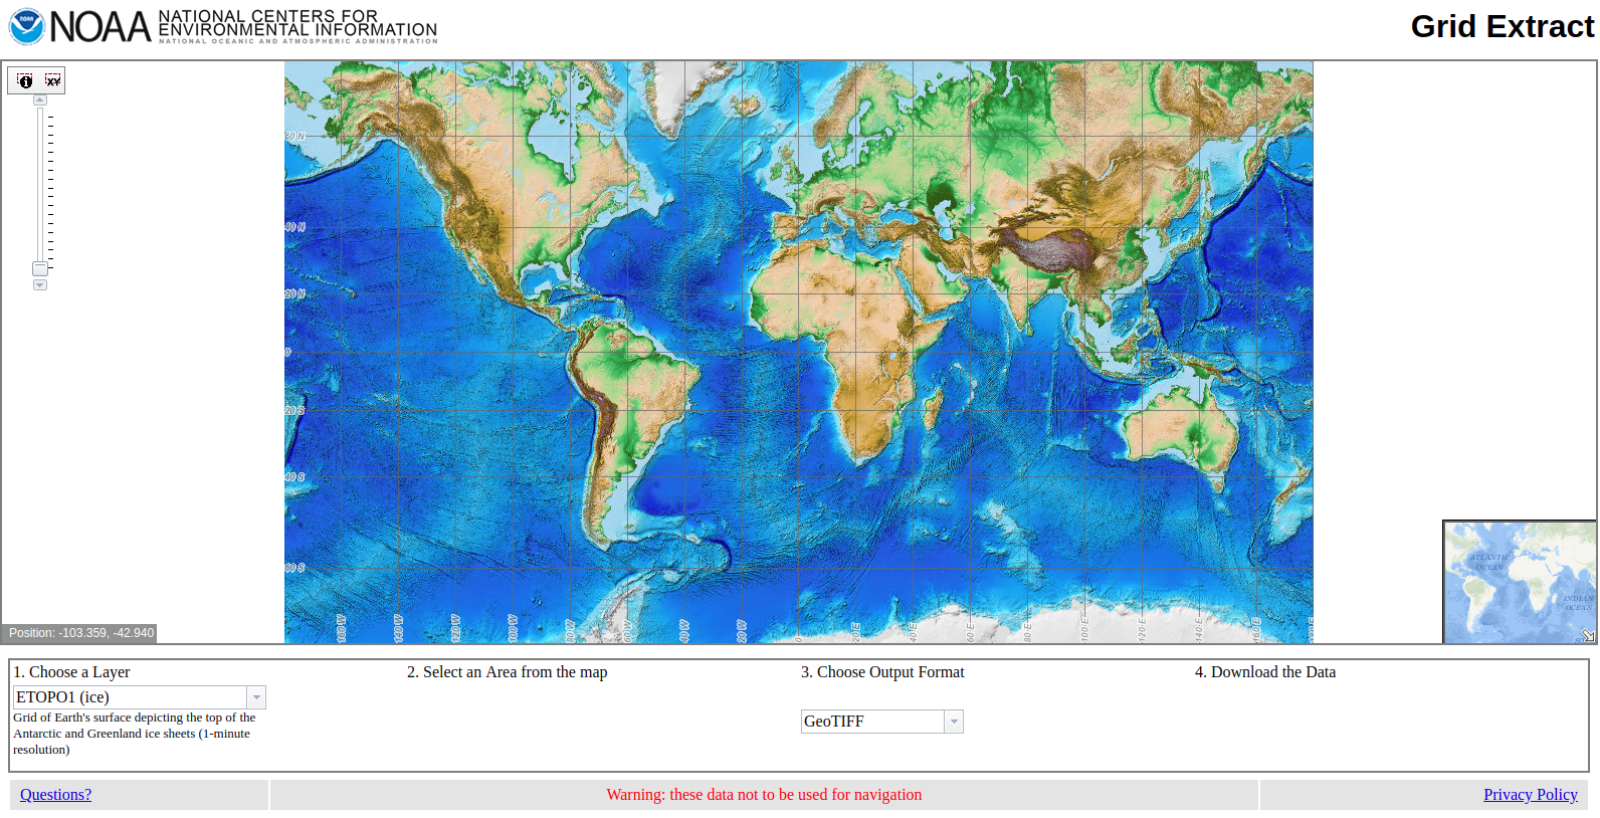
\includegraphics[width=0.85\textwidth]{etopo1.png}
    \caption{Apresentação do site do ETOPO1.}
    \label{etopo1}
\end{figure}
\bigskip

\noindent Com os dados do ETOPO1 baixados, abra o script \textit{make\_grid.py} para construir a grade do ROMS. E altere as variáveis de acordo com a Figura \textcolor{bleu_cite}{\ref{fazgrade}}.
\bigskip

\begin{figure}[H]
    \centering
    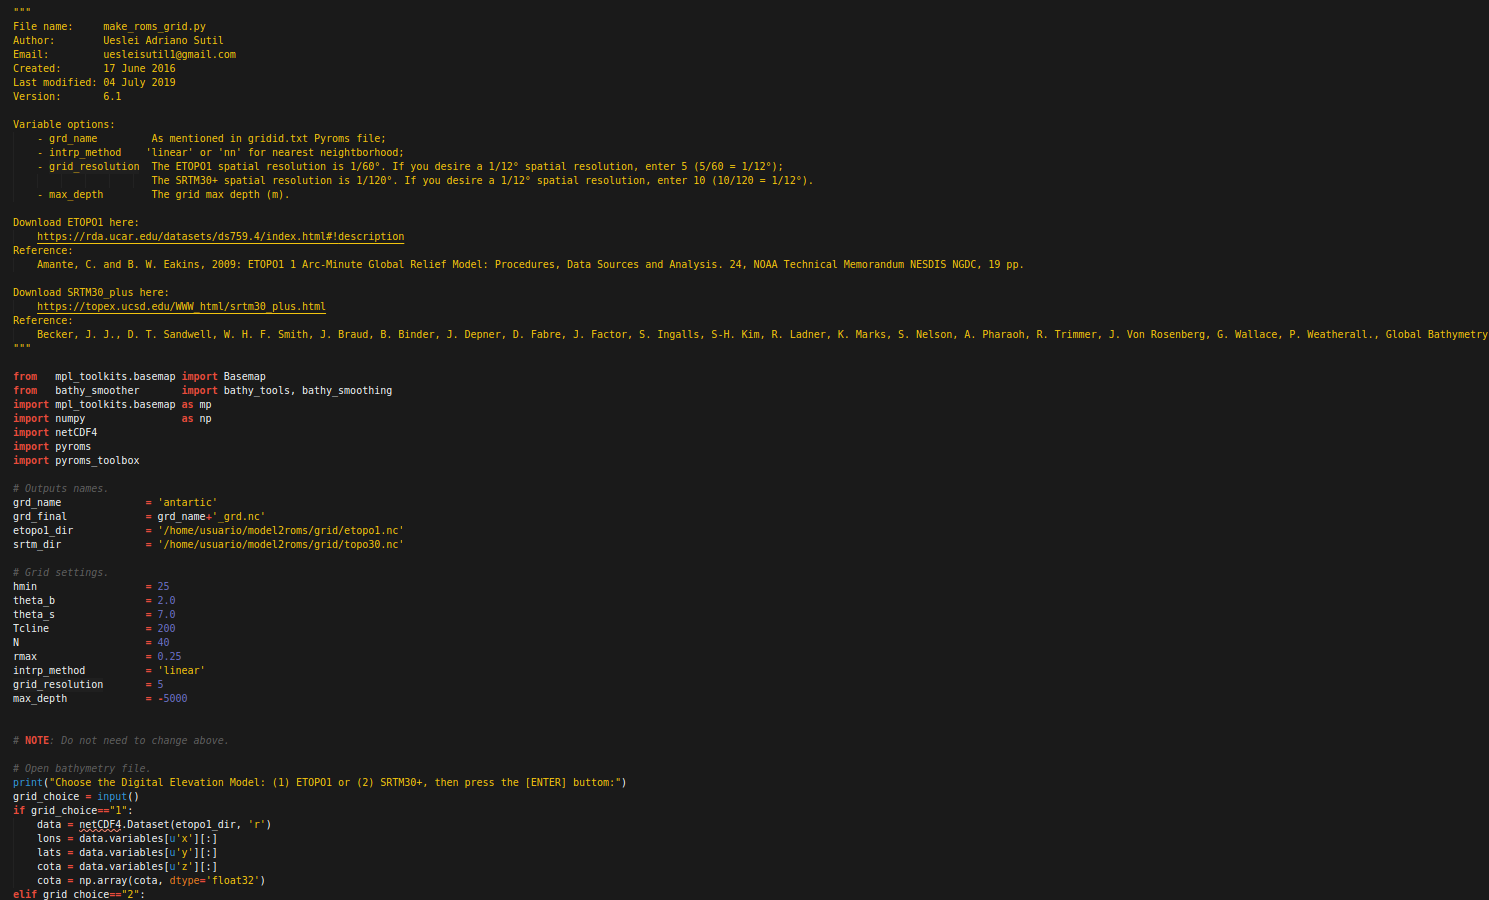
\includegraphics[width=0.70\textwidth]{makegrid.png}
    \caption{Captura de tela de parte do script \textit{make\_grid.py}, que se encontra dentro da pasta \textit{model2roms} no diretório de repositórios (\textit{/home/adriano.sutil/repositorio/model2roms}).}
    \label{fazgrade}
\end{figure}
\bigskip

\noindent É necessário delimitar os quatro pontos da grade com suas respectivas latitudes e longitudes, além de especificar as latitudes para o Basemap. É necessário colocar os diretórios de outputs e inputs. As configurações da grade do ROMS estão ordenadas como:
\bigskip

\begin{itemize}
\item \textbf{Lm}: Pontos de grade.
\item \textbf{Mm}: Pontos de grade.
\item \textbf{hmin}: Valor mínimo de h.
\item \textbf{theta\_b}: S-coordinate bottom  control parameter
\item \textbf{theta\_s}: S-coordinate surface control parameter
\item \textbf{Tcline}: Critical depth (hc) in meters (positive) controlling the stretching. It can be interpreted as the width of surface or bottom boundary layer in which higher vertical resolution.
\item \textbf{N}: Número de camadas Sigma;
\item \textbf{interp\_method}: Método de interpolação da grade: Interpolação linear (\textit{linear}) ou por Vizinho Próximo (\textit{nn}).
\end{itemize}
\bigskip

\noindent Abra o arquivo \textit{gridid.txt} e modifique os parâmetros no arquivo de acordo com o que está no arquivo \textit{make\_grid.py}. A mudança é necessária porque o PyROMS utiliza este arquivo para buscar as configurações de grade.
\bigskip

\noindent Após realizar as modificações, basta apenas rodar o script principal, digite no terminal:
\bigskip

\begin{bashcode}
ipython make_roms_grid.py --pylab
\end{bashcode}
\bigskip

\subsection{O Simple Ocean Data Assimilation (SODA)}\index{O Simple Ocean Data Assimilation (SODA)}
\bigskip

\noindent O \textit{model2roms} foi desenvolvido para gerar as condições do ROMS utilizando o \textit{Simple Ocean Data Assimilation} versão 3.7.1. O SODA é um conjunto de dados de reanálises desenvolvido por Carton e Giese (2008) e produzios por um modelo de circulação global dos oceanos e a partir de assimilação de dados observacionais oriundas de diversas fontes. Os dados do SODA possuem um campo global de grade de 0,5\degree x 0,5\degree, 40 níveis verticais e resolução temporal de 5 dias ou mensal.
\bigskip

\noindent Os dados a cada 5 dias do SODA se encontram no cluster Kerana no diretório:
\bigskip

\begin{bashcode}
/home/luciano.pezzi/SODA3.3.1
\end{bashcode}
\bigskip

\subsection{Gerar as condições do ROMS}\index{Gerar as condições do ROMS }
\bigskip

\noindent A \textit{toolbox} \textit{model2roms} completa se encontra dentro do repositório na Kerana. Para baixar, entre no diretório:
\bigskip

\begin{bashcode}
/home/adriano.sutil/repositorio/ROMS_scripts/model2roms
\end{bashcode}
\bigskip

\noindent Ao abrir a pasta do \textit{model2roms} é possível observar diversos scripts. Usaremos apenas o script \textit{config.py} e o \textit{compile.py}
\bigskip

\noindent Compile a \textit{toolbox} com o comando:
\bigskip

\begin{bashcode}
  ipython compile.py --pylab
\end{bashcode}
\bigskip

\noindent Abra o arquivo \textit{config.py} e, conforme a Figura \textcolor{bleu_cite}{\ref{editmaskgrid}}, pela definição \textit{defineromsgridpath}. \textit{ProjetoROMS} é o seu nome de projeto, portanto altere se achar conveniente. Em seguida altere o caminho onde está localizada a grade do ROMS. Em \textit{defineforcingdatapath}, altere o diretório onde se encontram os dados do SODA.

\begin{figure}[H]
    \centering
    \captionsetup{justification=centering}
    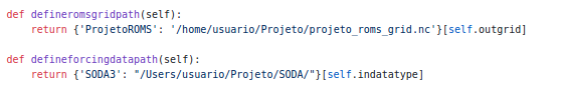
\includegraphics[width=0.82\textwidth]{1_grid_forcing.png}
    \caption{Caminhos para identificar o nome do projeto, a grade do ROMS e o diretório do SODA.}
    \label{editmaskgrid}
\end{figure}
\bigskip

\noindent Em seguida, faça alterações na guia \textit{EDIT} conforme desejado (Figura \textcolor{bleu_cite}{\ref{configmodel2roms}}), alterando entre \textit{True} ou \textit{False}.
\bigskip

\begin{itemize}
\item \textbf{\textit{self.showprogress}}: Mostra uma barra de progresso. Caso deseje utilizar, é necessário instalar o pacote \textit{progressbar2}. Instale através do Conda com o comando:
\end{itemize}
\bigskip
\begin{bashcode}
conda install -c anaconda progressbar2
\end{bashcode}
\bigskip

\begin{figure}[H]
    \centering
    \captionsetup{justification=centering}
    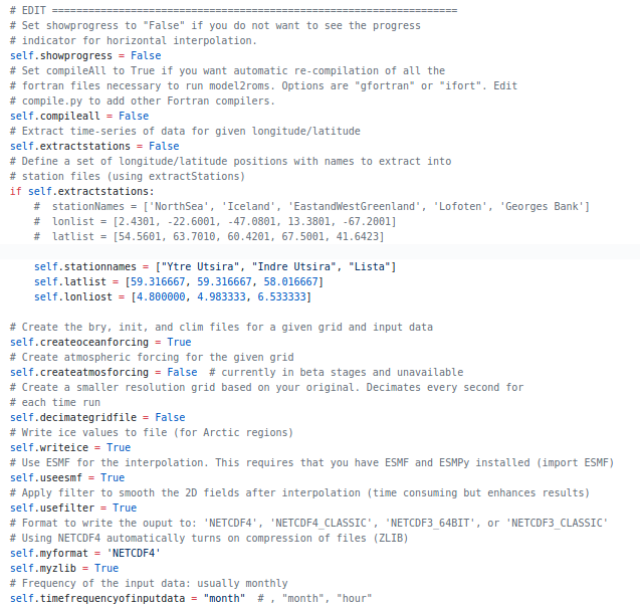
\includegraphics[width=0.85\textwidth]{1_defsmodel2roms.png}
    \caption{Definições para utilizar o \textit{model2roms} no script \textit{config.py}.}
    \label{configmodel2roms}
\end{figure}
\bigskip

\begin{itemize}
\item \textbf{\textit{self.compileall}}: Marque \textit{True} caso queira compilar automaticamente toda vez que utilizar a \textit{toolbox}.
\item \textbf{\textit{self.extractstations}}: Caso queira extrair os dados de estações, fornecendo a latitude e longitude dos pontos.
\item \textbf{\textit{self.createoceanforcing}}: Para criar as forçantes oceânicas.
\item \textbf{\textit{self.creatatmosforcing}}: Para criar as forçantes atmosféricas. Atualmente está em fase beta.
\item \textbf{\textit{self.decimategridfile}}: Cria uma nova grade com resolução menor que a atual.
\item \textbf{\textit{self.writeice}}: Caso a grade esteja em domínio com gelo, cria as variáveis para este fim.
\item \textbf{\textit{self.useesmf}}: Usa o \textit{ESMF} e o \textit{ESMPy} para interpolação.
\item \textbf{\textit{self.usefilter}}: Suaviza os campos 2D, porém consome mais tempo de processamento.
\item \textbf{\textit{self.myformat}}: Define qual o formato do arquivo \textit{netcdf}. Utilizar o formato \textit{NETCDF4} automaticamente ativa a biblioteca \textit{zlib}.
\item \textbf{\textit{self.timefrequencyofinputdata}}: Define a frequência dos dados do SODA.
\end{itemize}
\bigskip

\noindent Na guia \textit{IN GRIDTYPES} estão descritas as opções de entrada da grade e do SODA, conforme a Figura \textcolor{bleu_cite}{\ref{inputmodel2roms}}.
\bigskip

\begin{figure}[H]
    \centering
    \captionsetup{justification=centering}
    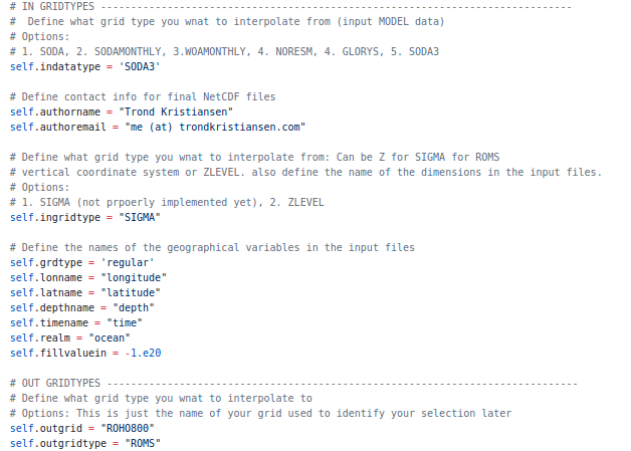
\includegraphics[width=0.85\textwidth]{1_inputgridtypes.png}
    \caption{Definições de entrada para utilizar o \textit{model2roms} no script \textit{config.py}.}
    \label{inputmodel2roms}
\end{figure}
\bigskip

\begin{itemize}
\item \textbf{\textit{self.indatatype}}: Seleciona qual a fonte de entrada dos dados.
\item \textbf{\textit{self.authorname}}: Escreve o nome do autor.
\item \textbf{\textit{self.authoremail}}: Escreve o email do autor.
\item \textbf{\textit{self.ingridtype}}: Define qual o tipo de grade do ROMS que será utilizada para gerar as condições.
\item \textbf{\textit{self.grdtype}}: Define qual o tipode grade que será criada.
\item \textbf{\textit{self.lonname}}: Define o nome da variável de longitude.
\item \textbf{\textit{self.depthname}}: Define o nome da variável de profundidade.
\item \textbf{\textit{self.timename}}: Define o nome da variável de tempo.
\item \textbf{\textit{self.realm}}: Informa que está criando os dados oceânicos ou atmosféricos.
\item \textbf{\textit{self.fillvaluein}}: Valor de \textit{fillvalue} utilizado nos arquivos \textit{netcdf}.
\end{itemize}
\bigskip

\noindent Na aba \textit{OUT GRIDTYPES} estão detalhados os dados de grade, conforme a figura \textcolor{bleu_cite}{\ref{outmodel2roms}}.
\bigskip

\begin{figure}[H]
    \centering
    \captionsetup{justification=centering}
    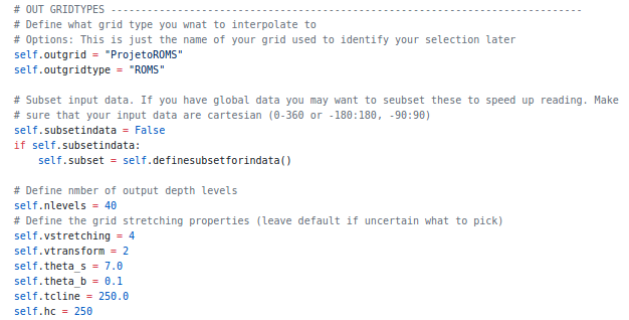
\includegraphics[width=0.85\textwidth]{1_outputgridtypes.png}
    \caption{Definições de saída para utilizar o \textit{model2roms} no script \textit{config.py}.}
    \label{outmodel2roms}
\end{figure}
\bigskip

\begin{itemize}
\item \textbf{\textit{self.outgrid}}: O nome do seu projeto do ROMS.
\item \textbf{\textit{self.outgridtype}}: O tipo de grade que será criado.
\item \textbf{\textit{self.nlevels}}: A quantidade de níveis verticais ds condições.
\item \textbf{\textit{self.vstretching}}: Número da opção da função de alongamento das coordenadas verticais.
\item \textbf{\textit{self.vtransform}}: Número da opção da função de transformaçoes de coordenadas verticais.
\item \textbf{\textit{self.theta\_s}}: Parâmetro usado para controlar as coordenadas na superfície.
\item \textbf{\textit{self.theta\_b}}: Parâmetro usado para controlar as coordenadas na camada inferior.
\item \textbf{\textit{self.tcline}}: Parâmetro usado para controlar a largura entre a camada superficial e interior.
\item \textbf{\textit{self.hc}}: Parâmetro utilizado para a camada crítica.
\end{itemize}
\bigskip

\noindent Na aba \textit{DATE AND TIME DETAILS} estão detalhados as datas de início e fim do experimento, conforme a Figura \textcolor{bleu_cite}{\ref{datetimemodel2roms}}.
\bigskip

\begin{figure}[H]
    \centering
    \captionsetup{justification=centering}
    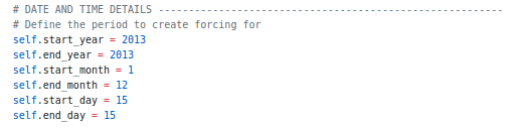
\includegraphics[width=0.85\textwidth]{1_timemodel2roms.png}
    \caption{Definições de datas para utilizar o \textit{model2roms} no script \textit{config.py}.}
    \label{datetimemodel2roms}
\end{figure}
\bigskip

\begin{itemize}
\item \textbf{\textit{self.start\_year}}: Ano inicial.
\item \textbf{\textit{self.end\_year}}: Ano final.
\item \textbf{\textit{self.start\_month}}: Mês inicial.
\item \textbf{\textit{self.end\_month}}: Mês final.
\item \textbf{\textit{self.start\_day}}: Dia inicial.
\item \textbf{\textit{self.end\_day}}: Dia final.
\end{itemize}
\bigskip

\noindent Agora, com os dados todos completados, basta executar a \textit{toolbox} com o comando:
\bigskip

\begin{bashcode}
ipython config.py --pylab
\end{bashcode}

\section{Acoplando o modelo de gelo marinho ao ROMS}
\bigskip